\chapter{El grupo fundamental}

\section{Homotopía por arcos}

\begin{definicion}
    Sean $X$ e $Y$ dos espacios topologicos y $f,g:X\to Y$ dos aplicaciones continuas. Decimos que $f$ es \textbf{homotópica} a $g$ si existe $H:X\times[0,1]\to Y$ continua tal que 
    \begin{gather*}
        H(x,0) = f(x) \hspace{0.5cm} \text{ y } \hspace{0.5cm} H(x,1) = g(x) \ \ \ \forall x\in X
    \end{gather*}

    \begin{figure}[H]
        \centering
        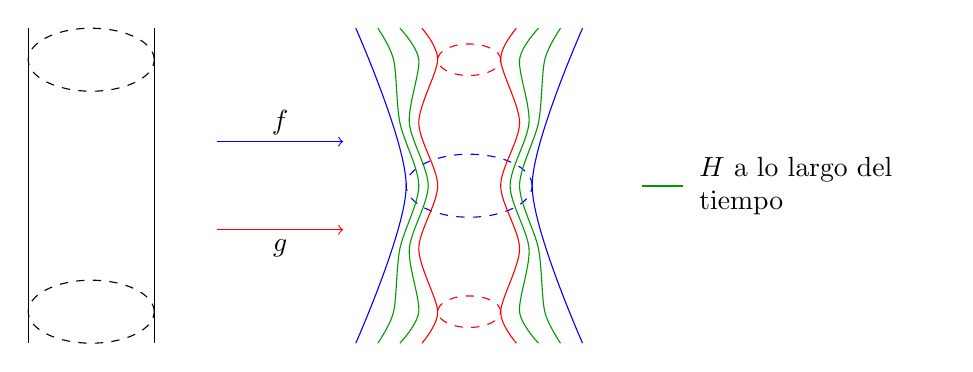
\begin{tikzpicture}[scale=0.8]
            \shorthandoff{>}

            % Cono 
            \draw[dashed] (-3,2) ellipse (1 and 0.5);
            \draw[dashed] (-3,-2) ellipse (1 and 0.5);

            \draw (-4,-2.5) -- (-4,2.5);
            \draw (-2,-2.5) -- (-2,2.5);

            % Flecha f
            \node at (0,1) {$f$};
            \draw[->, blue] (-1,0.7) -- (1,0.7);

            % Flecha g
            \node at (0,-1) {$g$};
            \draw[->, red] (-1,-0.7) -- (1,-0.7);

            % Leyenda H
            \node[text width=3cm, anchor=west] at (6.5,0) {$H$ a lo largo del tiempo};
            \draw[thick, green!60!black] (5.75,0)--(6.4,0);

            % Imagen de f
            \draw[dashed, blue] (3,0) ellipse (1 and 0.5);
            \draw[blue] plot[smooth] coordinates {
                (1.2,-2.5) (2,0) (1.2,2.5)
            };
            \draw[blue] plot[smooth] coordinates {
                (4.8,-2.5) (4,0) (4.8,2.5)
            };

            % Imagen de g
            \draw[dashed, red] (3,2) ellipse (0.5 and 0.25);
            \draw[dashed, red] (3,-2) ellipse (0.5 and 0.25);
            \draw[red] plot[smooth] coordinates {
                (2.25,2.5) (2.5,2) (2.2,1) (2.5,0) (2.2,-1) (2.5,-2) (2.25,-2.5)
            };
            \draw[red] plot[smooth] coordinates {
                (3.75,2.5) (3.5,2) (3.8,1) (3.5,0) (3.8,-1) (3.5,-2) (3.75,-2.5)
            };

            % Intermedios derecha
            \draw[green!60!black] plot[smooth] coordinates {
                (4.1,2.5) (3.8,2) (3.95,1) (3.65,0) (3.95,-1) (3.8,-2) (4.1,-2.5)
            };
            \draw[green!60!black] plot[smooth] coordinates {
                (4.45,2.5) (4.2,2) (4.1,1) (3.8,0) (4.1,-1) (4.2,-2) (4.45,-2.5)
            };

            % Intermedios izquierda
            \draw[green!60!black] plot[smooth] coordinates {
                (1.9,2.5) (2.2,2) (2.05,1) (2.35,0) (2.05,-1) (2.2,-2) (1.9,-2.5)
            };
            \draw[green!60!black] plot[smooth] coordinates {
                (1.55,2.5) (1.8,2) (1.9,1) (2.2,0) (1.9,-1) (1.8,-2) (1.55,-2.5)
            };


        \end{tikzpicture}
    \end{figure}

\end{definicion} 

\begin{definicion}
    Dados $X$ e.t., $x,y\in X$ y dos arcos $\alpha, \beta\in \Omega(X;x,y)$, decimos que $\alpha, \beta$ son \textbf{homotópicos por arcos} si existe $H:[0,1]\times [0,1] \to X$ continua tal que 
    \begin{align*}
        H(s,0) = \alpha(s) \hspace{0.5cm} &\text{ y } \hspace{0.5cm} H(s,1) = \beta(x) \ \ \ &\forall s\in [0,1]\\
        H(0,t) = x  \hspace{0.5cm} &\text{ y } \hspace{0.5cm} H(1,t) = y \ \ \ &\forall t \in [0,1]
    \end{align*}
\end{definicion}

\begin{lema}
    Ser homotópico por arcos da lugar a una relación de equivalencia en $\Omega(X;x,y)$.
    \begin{proof}\
        \begin{enumerate}
            \item[(i)] Dado $\alpha \in \Omega(X;x,y)$ queremos ver que $\alpha$ es homotópica por arcos con $\alpha$. Para ello tenemos 
            \begin{align*}
                H(s,t) = \alpha(s) \hspace{1cm} & H(s,0) = \alpha(s)=H(s,1)\\
                H(0,t) = \alpha(0)=x \hspace{1cm} & H(1,t) = \alpha(1) = y
            \end{align*}

            \item[(ii)] Dados $\alpha, \beta\in \Omega(X;x,y)$ tales que existe $H:[0,1]\times [0,1]\to X$ continua tal que 
            \begin{align*}
                H(s,0) = \alpha(s) \hspace{0.5cm} &\text{ y } \hspace{0.5cm} H(s,1) = \beta(x) \ \ \ &\forall s\in [0,1]\\
                H(0,t) = x  \hspace{0.5cm} &\text{ y } \hspace{0.5cm} H(1,t) = y \ \ \ &\forall t \in [0,1]
            \end{align*}
            Queremos ver que existe un $\tilde{H}:[0,1]\times[0,1]\to X$ continua tal que 
            \begin{align*}
                \tilde{H}(s,0) = \beta(s) \hspace{0.5cm} &\text{ y } \hspace{0.5cm} \tilde{H}(s,1) = \alpha(x) \ \ \ &\forall s\in [0,1]\\
                \tilde{H}(0,t) = x  \hspace{0.5cm} &\text{ y } \hspace{0.5cm} \tilde{H}(1,t) = y \ \ \ &\forall t \in [0,1]
            \end{align*}
            Tomando $\tilde{H}(s,t):=H(s, 1-t)$ cumple claramente con lo que buscamos.

            \item[(iii)] Dado $\alpha, \beta, \gamma\in \Omega(X;x,y)$ y $H_1,H_2:[0,1]\times[0,1]\to X$ continuas tales que 
            \begin{gather*}
                \begin{array}{l c|c l}
                    H_1(s,0) = \alpha(s) &&& H_2(s,0) = \beta(s)\\
                    H_1(s,1) = \beta(s) &&& H_2(s,1) = \gamma(s)\\
                    H_1(0,t) = x &&& H_2(0,t) = x\\
                    H_1(1, t) = x &&& H_2(1,t) = y
                \end{array}
            \end{gather*}
            Queremos ver que existe un $H:[0,1]\times [0,1]\to X$ tal que 
            \begin{align*}
                H(s,t) = \alpha(s) \hspace{1cm} & H(s,0) = \alpha(s)=H(s,1)\\
                H(0,t) = \alpha(0)=x \hspace{1cm} & H(1,t) = \alpha(1) = y
            \end{align*}
            Para ello consideramos 
            \begin{gather*}
                H(s,t) = \left\{
                    \begin{array}{l c c}
                        H_1(s,2t) & \text{ si } & 0 \leq t \leq \nicefrac{1}{2}\\
                        H_2(s, 2t-1) & \text{ si } & \nicefrac{1}{2} \leq t \leq 1
                    \end{array}
                \right.
            \end{gather*}
            Y con el lema de pegado es fácil ver que es continua y que satisface las condiciones que buscábamos.
        \end{enumerate}
    \end{proof}
\end{lema}

% TODO: Hacer lo mismo pero para homotopía

\begin{ejemplo}\
    \begin{enumerate}
        \item Sean $X$ un e.t. y $f,g:X \to \bb{R}^n$ aplicaciones continuas, entonces vamos a ver que $f$ y $g$ son homotópicas.
        \begin{proof}
            Vamos a definir la aplicación
            \begin{align*}
                H:X\times [0,1]&\to \bb{R}^n\\
                (x,t) & \mapsto (1-t)f(x) + tg(x)
            \end{align*} 
            que es continua y además verifica
            \begin{gather*}
                H(x,0) = f(x) \hspace{2cm} H(x,1) = g(x)
            \end{gather*}
            por lo que tenemos lo que buscábamos.
        \end{proof}
        En el caso particular de que $f=\alpha$ y $g=\beta$ fuesen arcos comenzando en un punto común y acabando en otro punto común, entonces la $H$ anterior sería una homotopía por arcos.

        \item Si $\alpha: [0,1]\to X$ es un arco y $h:[0,1] \to [0,1]$ es una aplicación continua con $h(0)=0$ y $h(1)=1$, entonces $\dot{\alpha}(s) = \alpha(h(s))$ es homotópica por arcos a $\alpha(s)$.
        
        \begin{proof}
            Es claro que $\dot{\alpha}$ es continua y existe una homotopía por arcos entre $\alpha$ y $\dot{\alpha}$ que es la siguiente
            \begin{gather*}
                H(s,t) = \alpha((1-t)s + th(s))
            \end{gather*}
            que es claramente continua y que verifica que 
            \begin{align*}
                H(s,0) = \alpha(s) \hspace{1cm} & H(s,1) = \alpha(h(s)) = \dot{\alpha}(s)\\
                H(0,t) = \alpha(0)=\dot{\alpha}(1) \hspace{1cm} & H(1,t) = \alpha(1) = \dot{\alpha}(1)
            \end{align*}
        \end{proof}
        Intuitivamente podemos entender esto como que no importa a qué velocidad se recorra una curva para ser homotópico por arcos.
    \end{enumerate} 
\end{ejemplo}

\begin{notacion}
    Como convenio a la clase de equivalencia de un arco $\alpha$ en $\Omega(X;x,y)$ lo denotaremos por $[\alpha]$.
\end{notacion}

\begin{lema}
    Dados dos arcos $\alpha_1, \alpha_2$ en $\Omega(X;x,y)$ y $\beta_1, \beta_2\in \Omega(X; y,z)$. Se verifica que si $[\alpha_1] = [\alpha_2]$, entonces $[\alpha_1\ast\beta_1] = [\alpha_2\ast\beta_2]$.

    \begin{proof}
        Tenemos que 
        \begin{gather*}
            (\alpha_1\ast\beta_1) = \left\{
                \begin{array}{l c c}
                    \alpha_1(2s) & \text{ si } & 0 \leq s \leq \nicefrac{1}{2}\\
                    \beta_1(2s-1) & \text{ si } & \nicefrac{1}{2} \leq s \leq 1
                \end{array}
            \right.\\\\
            (\alpha_2\ast\beta_2) = \left\{
                \begin{array}{l c c}
                    \alpha_2(2s) & \text{ si } & 0 \leq s \leq \nicefrac{1}{2}\\
                    \beta_2(2s-1) & \text{ si } & \nicefrac{1}{2} \leq s \leq 1
                \end{array}
            \right.
        \end{gather*}
        Además, sabemos que existen $H_1, H_2$ continuas tal que 
        \begin{gather*}
            \begin{array}{c c c c}
                H_1(s,0) = \alpha_1(s) &&& H_2(s,0) = \beta_1(s)\\
                H_1(s,1) = \beta_1(s) &&& H_2(s,1) = \beta_2(s)\\
                H_1(0,t) = x &&& H_2(0,t) = y\\
                H_1(1, t) = y &&& H_2(1,t) = z
            \end{array}
        \end{gather*}
        Tomamos entonces $H:[0,1]\times [0,1] \to X$ dada por 
        \begin{gather*}
            H(s,t) = \left\{
                \begin{array}{l c c}
                    H_1(2s, t) & \text{ si } & s \in [0,\nicefrac{1}{2}],\ t\in [0,1]\\
                    H_2(2s-1, t) & \text{ si } & s \in [\nicefrac{1}{2},1],\ t\in [0,1]\\
                \end{array}
            \right.
        \end{gather*}
        es continua y tenemos que 
        \begin{gather*}
            H(s,0) = \left\{
                \begin{array}{l c c}
                    H_1(2s, 0) & \text{ si } & s \in [0,\nicefrac{1}{2}]\\
                    H_2(2s-1, 0) & \text{ si } & s \in [\nicefrac{1}{2},1]\\
                \end{array}
            \right. = 
            \left\{
                \begin{array}{l c c}
                    \alpha_1(2s) & \text{ si } & s \in [0,\nicefrac{1}{2}]\\
                    \beta_1(2s-1) & \text{ si } & s \in [\nicefrac{1}{2},1]\\
                \end{array}
            \right. = (\alpha_1 \ast \beta_1)(s)
        \end{gather*}
        Análogamente se tiene que $H(s,1)=(\alpha_2\ast\beta_2)(s)$ con $H(0,t) = x$ y $H(1,t) = z$.

    \end{proof}
    A partir del lema anterior podemos definir
    \begin{gather*}
        [\alpha] \ast [\beta] := [\alpha \ast \beta]
    \end{gather*}
    con $\alpha\in \Omega(X;x,y)$, $\beta \in \Omega(X;y,z)$
\end{lema}

\begin{teo} %TODO: Arreglar el cacho de enmedio (segunda parte de la demostración)
    Dado $X$ e.t., $\alpha\in \Omega(X;x,y)$, $\beta\in \Omega(X;y,z)$ y $\gamma\in \Omega(X;z,w)$ se tiene que 
    \begin{enumerate}
        \item[(i)] $[\alpha] \ast ([\beta] \ast [\gamma]) = ([\alpha] \ast [\beta]) \ast [\gamma]$
        \item[(ii)] $[\alpha]\ast [\veps_y] = [\alpha]$ y $[\veps_x]\ast [\alpha] = [\alpha]$
        \item[(iii)]  $[\alpha]\ast [\tilde{\alpha}] = [\veps_x]$ y $[\tilde{\alpha}]\ast [\alpha] = [\veps_y]$
    \end{enumerate}
    \begin{proof}\
        \begin{enumerate}
            \item[(i)] Desarrollemos lo que estamos calculando
            \begin{align*}
                (\beta\ast\gamma)(s) &= \left\{
                    \begin{array}{l c c}
                        \beta(2s) & \text{ si } & s \in [0,\nicefrac{1}{2}]\\
                        \gamma(2s-1) & \text{ si } & s \in [\nicefrac{1}{2},1]\\
                    \end{array}
                \right.\\\\
                \alpha \ast(\beta\ast\gamma)(s) &= \left\{
                    \begin{array}{l c c}
                        \alpha(2s) & \text{ si } & s \in [0,\nicefrac{1}{2}]\\
                        (\beta\ast\gamma)(2s-1) & \text{ si } & s \in [\nicefrac{1}{2},1]\\
                    \end{array}
                \right. =\\
                &= \left\{
                    \begin{array}{l c c}
                        \alpha(2s) & \text{ si } & s \in [0,\nicefrac{1}{2}]\\
                        \beta(2(2s-1)) & \text{ si } & s \in [\nicefrac{1}{2},\nicefrac{3}{4}]\\
                        \gamma(2(2s-1)-1) & \text{ si } & s \in [\nicefrac{3}{4},1]\\
                    \end{array}
                \right. = \left\{
                    \begin{array}{l c c}
                        \alpha(2s) & \text{ si } & s \in [0,\nicefrac{1}{2}]\\
                        \beta(4s-2) & \text{ si } & s \in [\nicefrac{1}{2},\nicefrac{3}{4}]\\
                        \gamma(4s-3) & \text{ si } & s \in [\nicefrac{3}{4},1]\\
                    \end{array}
                \right.\\\\\\
                %
                %
                %
                (\alpha\ast\beta)(s) &= \left\{
                    \begin{array}{l c c}
                        \alpha(2s) & \text{ si } & s \in [0,\nicefrac{1}{2}]\\
                        \beta(2s-1) & \text{ si } & s \in [\nicefrac{1}{2},1]\\
                    \end{array}
                \right.\\\\
                (\alpha \ast\beta)\ast\gamma(s) &= \left\{
                    \begin{array}{l c c}
                        (\alpha\ast\beta)(2s) & \text{ si } & s \in [0,\nicefrac{1}{2}]\\
                        \gamma(2s-1) & \text{ si } & s \in [\nicefrac{1}{2},1]\\
                    \end{array}
                \right. =\\
                &= \left\{
                    \begin{array}{l c c}
                        \alpha(2(2s)) & \text{ si } & s \in [0,\nicefrac{1}{4}]\\
                        \beta(2(2s)-1) & \text{ si } & s \in [\nicefrac{1}{4},\nicefrac{1}{2}]\\
                        \gamma(2s-1) & \text{ si } & s \in [\nicefrac{3}{4},1]\\
                    \end{array}
                \right. = \left\{
                    \begin{array}{l c c}
                        \alpha(4s) & \text{ si } & s \in [0,\nicefrac{1}{4}]\\
                        \beta(4s-1) & \text{ si } & s \in [\nicefrac{1}{4},\nicefrac{1}{2}]\\
                        \gamma(2s-1) & \text{ si } & s \in [\nicefrac{1}{2},1]\\
                    \end{array}
                \right.
            \end{align*}
            Usando el ejemplo 2 anterior se tiene que $[\alpha] \ast ([\beta] \ast [\gamma]) = ([\alpha] \ast [\beta]) \ast [\gamma]$
        \end{enumerate}
    \end{proof}
\end{teo}